\chapter{Redes}\label{S:anexo_D}
Este anexo muestra el razonamiento y pruebas de concepto realizadas durante el tema 3 de  redes.

\section{Conceptos básicos}

Para entender la naturaleza de las redes informáticas así como el servicio que brinda una VPN, inicialmente hay que tener un contexto y conceptos básicos. Una red es un conjunto de dispositivos informáticos interconectados por medio físico o inalámbrico. Para la apropiada conexión y gestión de las comunicaciones entre los dispositivos existe una infraestructura, cables, routers, switch, antenas así como identificadores y software interrelacionados.

\begin{figure}[!htb]
\begin{center}
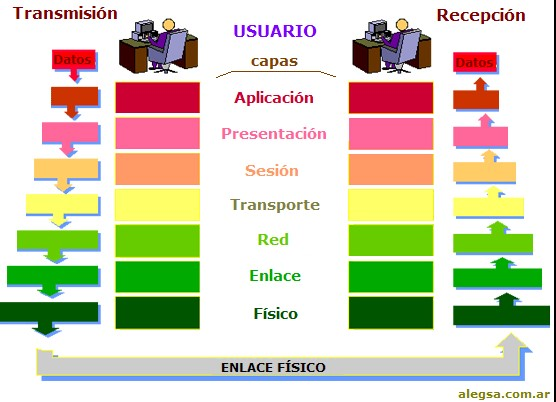
\includegraphics[width=0.7\textwidth]{./figuras/capas_osi}
\caption{Diagrama capa OSI \cite{c_osi}.}
\label{F:capas_osi}
\end{center}
\end{figure}

Para entender la comunicaciones dentro de una red, se necesita el modelo de la capa OSI\cite{c_osi} así como nociones básicas de la capa física (cables, antenas, hubs, ethernet) y de la capa de enlace (L2) como protocolos arp, icmp e identificadores MAC.

Podemos resumir brevemente que la capa L1 físico, es propiamente el hardware y la manera 'física' de comunicarse a través de señales electromagnéticas, procesar las señales y software-drivers de dicho hardware.

La capa L2 o Enlace, se refiere al conjunto de protocolos, identificadores que permiten la comunicación y repetición de comunicaciones de elementos conectados físicamente.

La capa L3 o de red, son los protocolos, identificadores y funcionalidades (enrutar, nat, dns ...) que auxilian, permiten y realizan el envió de paquetes a través de una red. 

La capa L4 o transporte son principalmente protocolos de transporte, permiten verificar y optimizar la transmisión de paquetes entre elementos de la red.

El resto de capas superiores se focalizan en la seguridad, protocolos de aplicación o los datos intrínsecos.

Cuando hablamos de transmisión de datos en una red, hablamos de 'paquetes' es decir conjuntos organizados de datos. Estos paquetes se organizan a capas siguiendo las funciones de la pila OSI, por lo tanto para cada nivel existen una cabeceras y una carga útil de datos que contiene niveles superiores.

Un punto importante a entender es que no existe una única red, sino multitud de redes, las cuales están interconectadas entre si. A el conjunto de redes publicas interconectadas entre si es lo que hoy en día llamamos Internet, a los subconjuntos de redes privadas no publicas se les denomina intranet o red privada, y aquellas mono-redes privas locales que disponemos en nuestro router de casa se les denomina LANs (Local Area Network).

Es importante entender que el principal objetivos de este trabajo en temática de redes es configurar adecuadamente nuestras LANs en casa en conjunción con una red privada virtual (VPN) de carácter profesional, o la interconexión de LANs mediante VPN.

\subsection{VPN y encapsulado}
Una VPN es una red privada, virtual, es decir no tiene capa física real sino que es emulada. Para emular dicha capa se puede utilizar opciones de hardware especificas de fabricantes o un software. Nuestro caso software implica que usaremos una red real, sobre la cual se utilizara un servicio o aplicación de VPN, es decir, los paquetes de datos que se envían dentro de una VPN, son paquetes encapsulados en la capa de datos de aplicación.

\begin{figure}[!htb]
\begin{center}
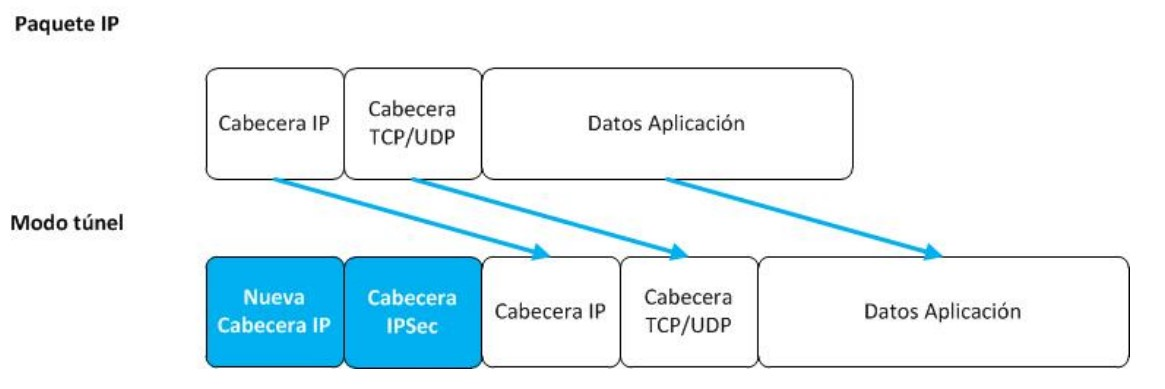
\includegraphics[width=0.9\textwidth]{./figuras/tunel_paneque}
\caption{Encapsulado túnel paquete de  VPN en red real.}
\label{F:tunel_paneque}
\end{center}
\end{figure}

Esta virtualiación puede degradar la condiciones respecto a la red real, especialmente por que los protocolos de transporte, no son capaces de ajustarse, al estar funcionando virtualizada mente sobre otra red.

\subsection{Protocolo y tecnología}
Actualmente existen múltiples opciones donde una política de confianza, mantenimiento o facilidad de configuración en uno y otro software es el desencadenante para su elección. Como soluciones validadas y evaluadas se han utilizado las siguientes tecnologías:

\subsubsection{Openswan / libreswan}
Ipsec\cite{c_ipsec} vpn, basada en un conjunto de protocolos de los 90 extendido bajo en nombre de librewan o openswan que permite hacer túneles p2p, principalmente estáticos, no dispone de interfaz gráfica y tiene una configuración compleja.

 Su principal ventaja es la sencillez de ser nativo y robusto, mientras su principal desventaja es su complejidad para poder pasar un firewall o NAT. Por lo que únicamente lo utilizaremos para túneles estáticos sobre elementos públicos, aunque es posible su configuración, requiere de un conocimiento previo así como no es user-friendly . Su principal característica es rapidez y simplicidad entre ip públicas.

 \subsubsection{OpenVPN y derivados}
 Openvpn\cite{c_openvpn}, es una conjunto de protocolos y software server/cliente con más de 15 años, en definitiva todo un estándar, estable, fácil de usar, pensado para evadir firewall y NATs. Su principal desventaja es que no es nativo, es decir requiere de instalación en ambos server y cliente, así como la velocidad del mismo no es a nivel de kernel del SO, por lo que induce un delay que degrada la condiciones de la conexión vpn, especialmente cuando utiliza TCP como protocolo de transporte. Su principal característica es su uso extensivo.

\subsubsection{Wireguard y derivados}
 Wireguard\cite{c_wireguard}, más moderno (2015) es prácticamente una mejora sobre los dos anteriores. Incluye la totalidad de las funcionalidades de openvpn al igual que permite una ejecución pseudo-nativa en kernel en el servidor. Requiere instalar tanto servidor como cliente ya que no es un protocolo incluido en los SO. Desde 2020 es estable y el actual reemplazo como protocolo estándar de vpn por lo que actualmente es la opción óptima.

\subsubsection{Otros protocolos}
Otros, existen software del nivel y calidad de wireguard, incluso más enfocados a conexiones p2p o descentralizadas como freelan, cjdns, o mejoras sobre protocolos antiguos vulnerados como sstp (mejora sobre pptp). Todos ellos tienen un factor en común, no son de amplio uso y por lo tanto su configuración, instalación y mantenimiento, no es simple y tiende a generar más problemas así como un soporte y documentación más reducido y menos actualizada. Por lo que no son adecuados para todos los públicos.

\subsubsection{VPN as Service}
Por último existen una multitud de servicios y software licenciado gratuito en sheft-host basado en openvpn, wireguard y combinaciones, especialmente en el área de clientes y gestión web-gráfica del servidor y las redes vpn. Sin embargo los más usados como “netmaker”\cite{c_netmaker}, requieren de unos recursos y herramientas “sobredimensionadas” ya que se centran en calidad y facilidad al cliente final y exceden nuestros recursos añadiendo complejidad adicional.

Por ello este documento centra sus pruebas de concepto en estos dos conjuntos de protocolos, \textbf{openvpn} y especialmente \textbf{wireguard} por su rapidez, en combinación con interfaces gráficas o gestores sencillos, asi como su gran uso, incluido por ejemplo en multitud de routers, televisores de manera nativa.

\subsection{Enrutado}\label{S:enrutado_sedes}
Debemos entender que todo elemento de una red es susceptible de estar interconectado en paralelo a otras redes, es decir, en un nodo con múltiples interfaces. Si dicho elemento permite el enrutado entre redes, puede recibir y reenviar paquetes entre ambas redes, esta propiedad es conocida en sistemas linux como ip forwarding.

Cuando nos conectamos a una red, se proveen de varios parámetros uno de ellos es el default gateway, es decir, la ruta por defecto. Normalmente tiene el valor de la IP del router (dentro de una LAN-NAT), puesto que para salir al exterior se debe enviar los paquetes al router. Sin embargo existe la posibilidad de añadir más rutas en “la tabla de enrutado”. 

Existen multitud de protocolos (RIP, OSPF, BGP..) para transmitir qué redes son accesibles a través de qué nodo y añadir las rutas predefinidas en la tabla de enrutado. Pero no es el objetivo de este trabajo, por lo que para los casos de uso actual utilizaremos enrutamientos estáticos añadidos, es decir, modificar en los router, vpn server o clientes vpn la tabla de enrutado para permitir la intercomunicación de redes. Ejemplo de 2 sedes y red en la nube interconectadas:
\begin{figure}[!htb]
\begin{center}
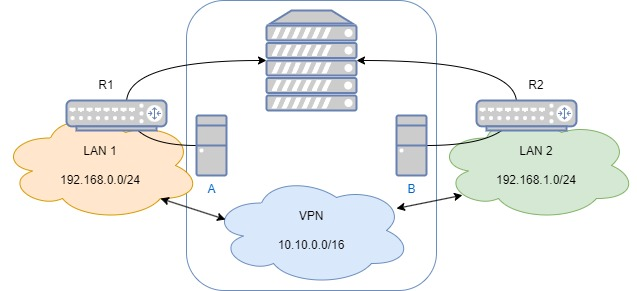
\includegraphics[width=0.8\textwidth]{./figuras/interconexion_redes}
\caption{Diagrama interconexión de redes por vpn.}
\label{F:interconexion_redes}
\end{center}
\end{figure}

Por ejemplo desde un elemento en la red naranja la tabla de enrutado es la siguiente:
\begin{table}[htb]
\begin{center}
\label{T:tabla_enrutado__redNaranja}
\caption{Tabla enrutado elemento solo conectado a la red naranja.}
\begin{tabular}{|l|c|c|}
\hline \hline
\multicolumn{1}{|c|}{Destino} & Interfaz   & Pasarela           \\ \hline
default / 0.0.0.0             & naranja    & R1.naranja \\ \hline
192.168.0.0/24                & naranja    & destinatario.naranja      \\ \hline
192.168.1.0/24                & naranja    & A.naranja          \\ \hline
10.10.0.0/16                  & naranja    &  A.naranja        \\ \hline
\end{tabular}
\end{center}
\end{table}
Es decir el router R1 gestiona todas las peticiones dentro y fuera de la red naranja a excepción de las peticiones a la red verde y azul, que son redirigidas al elemento A, conectado con la red azul(vpn) y a través de esta a vía la red verde.

\begin{table}[htb]
\begin{center}
\label{T:tabla_enrutado_A}
\caption{Tabla enrutado desde A.}
\begin{tabular}{|l|c|c|}
\hline \hline
\multicolumn{1}{|c|}{Destino} & Interfaz  & Pasarela           \\ \hline
default / 0.0.0.0             & A.azul    & azul vpn server ip \\ \hline
192.168.0.0/24                & A.naranja & destinatario.naranja     \\ \hline
192.168.1.0/24                & A.azul    & B.azul          \\ \hline
10.10.0.0/16                  & A.azul    & azul vpn server ip         \\ \hline
\end{tabular}
\end{center}
\end{table}

Queda patente que en la tabla de enrutado del elemento A este 'sale a internet' a través de la red VPN, lo cual es coherente puesto que su red principal es la VPN, aunque como se explico en figura \ref{F:tunel_paneque}, dichos paquetes son encapsulados dentro de paquetes que si utilizan la tabla de enrutado de la red naranja, por que físicamente salen a través del R1.
Desde la red verde podemos hacer observaciones equivalentes:

\begin{table}[htb]
\begin{center}
\label{T:tabla_enrutado_red_verde}
\caption{Tabla enrutado desde un elemento solo conectado a la red verde.}
\begin{tabular}{|l|c|c|}
\hline \hline
\multicolumn{1}{|c|}{Destino} & Interfaz  & Pasarela           \\ \hline
default / 0.0.0.0             & verde     & R2.verde \\ \hline
192.168.0.0/24                & verde     & A.azul.ip      \\ \hline
192.168.1.0/24                & verde     & destinatario.verde          \\ \hline
10.10.0.0/16                  & verde     & B.verde         \\ \hline
\end{tabular}
\end{center}
\end{table}

Similar al caso de A, B tiene como red principal y gateway la VPN, que es por donde sale a internet. En ambos casos A  y B utilizan su segunda interfaz conectada a la red azul, para enrutar paquetes dirigidos a la red azul o a redes que azul permite conectarse, y en contrapartida cuando algún paquete les llega desde la red azul hacia sus redes (naranja y verde) lo enrutan internamente. Son por lo tanto la "gateway" de interconexión en sus respectivas redes locales hacia el resto de redes de la intranet.

\begin{table}[htb]
\begin{center}
\label{T:tabla_enrutado_B}
\caption{Tabla enrutado desde B.}
\begin{tabular}{|l|c|c|}
\hline \hline
\multicolumn{1}{|c|}{Destino} & Interfaz  & Pasarela           \\ \hline
default / 0.0.0.0             & B.azul    & azul vpn server ip \\ \hline
192.168.0.0/24                & B.azul    & A.azul     \\ \hline
192.168.1.0/24                & B.verde   & destinatario.verde          \\ \hline
10.10.0.0/16                  & B.azul     & azul vpn server ip         \\ \hline
\end{tabular}
\end{center}
\end{table}

Con estas configuraciones cualquier elemento que conectemos a cualquiera de las 3 redes (naranja, azul o verde) tendrá acceso a ellas y por lo tanto es similar a estar todos en una única red privada, una intranet.

Entiéndase que un elemento ajeno a las sedes (trabajador teletrabajando) que se conecte únicamente a la red azul VPN, sin exponer su propia LAN, a la vez que también tendrá acceso a las 3 redes al ser un elemento de una de ellas.

\subsection{Nat Masquerade}
Cuando una red es privada, es decir no pública, significa que la numeración IP es propia y no se expone a internet. Por lo tanto no es accesible desde fuera, y de igual manera si intentamos acceder a internet mediante un mecanismo de salida, los paquetes ip nunca regresaran puesto que nuestra dirección remitente IP es privada.

Es un problema similar a enviar una carta sin remitente porque vivimos en una zona no urbana, o de difícil acceso. Normalmente se utiliza un apartado de correos, o una dirección pública existente, donde recibir la contestación.

La solución a este problema se llama nat-masquerade, y consiste exactamente en eso, nuestro router adsl/fibra está conectado a un ISSP y el si tiene una dirección pública como nuestro “apartado de correos”. El router genera nuestra red privada LAN e implanta un mecanismo de reemplazo de las cabecera IP, con el objetivo de que toda petición a internet sea él quien aparece como remitente y cuando la contestación es recibida, la enruta hace la fuente original.

Este mecanismo es el más habitual para interconectar redes privadas y públicas manteniendo la conectividad hacia afuera, pero negando la conectividad desde fuera de la red, únicamente se puede acceder al router que genera el NAT(Network Address Translation) o contestaciones a peticiones iniciadas desde dentro de la LAN.

Un caso especial son las ISP CG-NAT\cite{c_cg_nat}, que indica que la red de nuestro proveedor de internet también es privada, por lo que en realidad estamos navegando desde dos capas de NAT consecutivas.

\subsection{DNS}\label{S:dns}
DNS o sistema de nombres de dominio, es el servicio de red que nos permite traducir una URL “www.dominio.es” por la correspondiente IP a la que enviar nuestros paquetes. Es de especial importancia ya que aunque estemos conectados correctamente a una red con acceso a internet, sin el apropiado acceso a un dns, creeremos no tener internet ya que las peticiones en “lenguaje humano” no serán resultas.
\begin{figure}[!htb]
\begin{center}
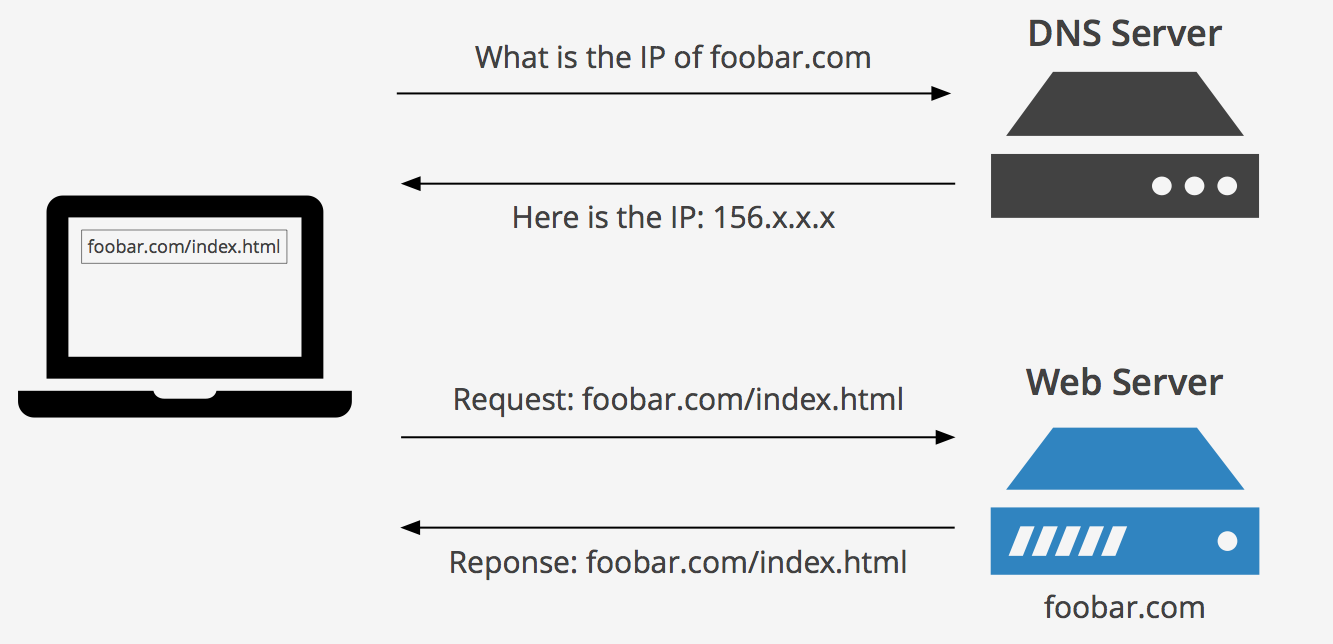
\includegraphics[width=0.9\textwidth]{./figuras/dns_resolution}
\caption{Diagrama resolución de queries dns proxy\cite{i_dns}.}
\label{F:dns_resolution}
\end{center}
\end{figure}
Los DNS permiten no sólo la traducción sino el balanceo de carga, el filtrado de peticiones y la monitorización del tipo de tráfico a través de las peticiones dns. 
Un DNS interno, suele ser un dns relay o proxy, es decir, un punto de repetición hacia un dns exterior que incluye el mapeado de dominios internos de nuestra redes privadas, para permitir resolver dominios privados.

El objetivo principal es que aquellas peticiones tales como, ‘webempresaria.internal’, ‘dropbox.internal’, ‘email.internal’, ‘productoA.internal’ puedan resolverse solas sin necesidad de saber la ip o ips indicadas, ya que esta puede ser dinámicas  y no depender de una puesta en marcha estática.

Es de especial interés ya que docker permite la generación de redes privadas entre el host y los container. Con el objetivo de evitar el uso de ip internal variables, implementa un sistema interno dns permitiendo el acceso a los container de múltiples formas, nombre, alias de red, hostname del container, identificador del container, ip internas de docker y el mapeo de puertos directamente en la host de docker.

Por ejemplo al configurar un wordpress y su db, como es una configuración que no debe depender de las ip asignadas, se utilizan estas resolución del nombre del container como ip de los servicios.

Existen herramientas como pi hole\cite{c_pi_hole}, adguard, nextdns que sobre escriben dominios reales o inspeccionan la queries dns bloqueando anuncios, spam o llamadas inseguras.

\subsection{Proxy}\label{S:proxy_reverse}
Un Proxy es un elemento intermediario, es decir, similar al concepto de nat, utilizar un elemento de la red para que envié y reciba los paquetes por nosotros.

Si es utilizado por los clientes, aquellos servicios que reciben las peticiones creen que es el proxy quien las realiza. Esta casuística era muy común en los 90, ya que debido a las bajas velocidades de conexión (15-64 kbps) recurrente mente se utilizaban un proxy-cache en empresas con el objetivo de obtener información previamente cacheada y optimizar tiempo y recursos. Actualmente se utiliza como método para enmascarar tu geo-ip o para tener acceso a servicios no disponibles en tu zona geográfica.

Si es utilizado por los servidores se le denomina reverse-proxy, ya que funciona de manera invertida. Los clientes realizan múltiples peticiones a un único proxy expuesto públicamente, el proxy identifica las peticiones y las redirige internamente a los servidores de los diferentes servicios. Principalmente permite balancear flujos, añadir https por redirección, centralizar las conexiones y aplicar filtros previos para rechazar peticiones sin usar recursos en los servidores.

\subsubsection{Let's Encrypt Https}
Actualmente todas las paginas web o servicios "profesionales" y especialmente seguros requieren de TLS (Transport Layer Segurity) o focalizados en peticiones web HTTPS\cite{c_https}.

Para implementar el HTTPS es necesario el uso de certificados, dichos certificados si queremos que sean confiables, es decir de utilidad publica, deben estar registrados o emitidos por entes confiables. Actualmente solicitar un certificado puede costar de 6-15€, pero el servicio de Let's Encrypt\cite{c_letsencrypt} provee de certificados temporales (3 meses) validos y gratuitos para dominios concretos.

\begin{figure}[!htb]
\begin{center}
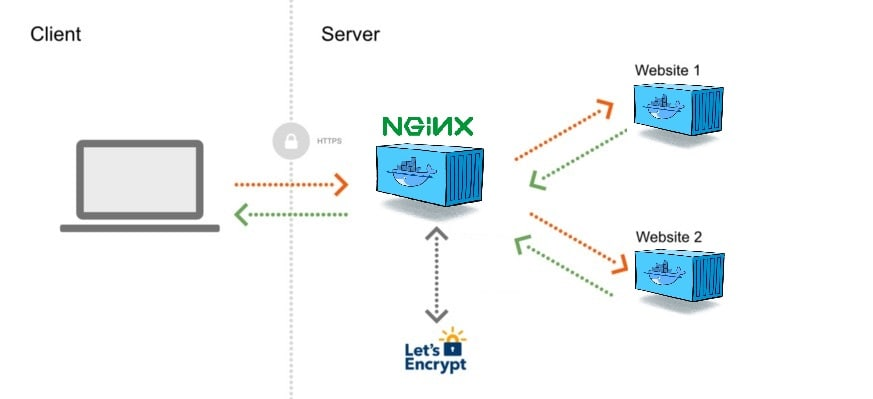
\includegraphics[width=0.9\textwidth]{./figuras/webproxy}
\caption{Ngix-rever proxy + Let's encrypt dockerized\cite{i_ngix_proxy}.}
\label{F:webproxy}
\end{center}
\end{figure}

Con el objetivo de que todas nuestras paginas publicas sea aceptadas por los navegadores y confiables se utilizara una estrategia de proxy-reverse basada en ngix y un bot automatizado de Let's encrypt que crea y actualiza los certificados que utiliza el reverse proxy.

\section{Seguridad}
La seguridad natural de una red se consigue por 3 métodos:
\begin{itemize}
    \item Dificultad o fortaleza de acceso, aquellas redes con protocolos de autenticación más robustos (certificados, algoritmo wireless seguros WPA2-AES), uso de cifrados temporales o medios físicos (cable, roseta) limitados, dificultan o impiden un acceso no autorizado al medio. 
    \item Limitación de acción o autorización por identificadores. Una manera de incrementar esta dificultad puede ser un filtrado de MAC (L2), o autenticación (L3 o superiores) para poder tener acceso real a los recursos de la red.  Desgraciadamente existen métodos de clonado e interceptación que permiten engañar a al red, pudiendo suplantar identificadores (MAC, IP) así como suplantar elementos una vez se tiene acceso a la red. 
    \item Limitación de comunicaciones por capas y sub-áreas de la red, el uso de VLAN, switch (L2) que limita las comunicaciones L1, router (L3) que limita las comunicaciones L2 es importante ya que una red jerárquica que aísla las diferentes capas OSI en sub-areas es mas robusta ante un ataque de suplantación, ya que únicamente un porcentaje de las comunicaciones de las red total es accesible en las diferentes capas. Por otra parte ataques masivos que bloquean las capacidades de la red, no son efectivos puesto únicamente afecta a segmentos parciales. Especialmente menciónale que elementos como WIFI, no permiten separar capas L1-L2-L3, siendo vulnerables, ya que una vez conseguido desencriptar el canal de , se pueden acceder a las otras dos capas.
\end{itemize}

Existen otros métodos activos, como escaneo y monitorización de la propia red para poder identificar intrusos pero no son objetivo de este trabajo.

\subsection{VLAN}\label{S:vlan}
VLAN o virtual LAN, es un mecanismo de generaciones de LAN virtuales.
Inicialmente se implemento por puerto, es decir, permitir utilizar los mismos elementos físicos (switch, router) en múltiples LAN sin interactuar entre ellas, creando una segregación de los puertos o cables (L1) que permite convivir múltiples Lan virtuales, sobre una única red física.

También existe un concepto similar a L2, por filtrado de MAC asignado en las diferentes VLAN. Usualmente VLAN se utiliza para cortar o aislar las comunicaciones L2, por ejemplo dentro de una misma LAN-router que dispone de conexiones cableada y wireless.

Desde la aparición de Ipv6, también puede segregar en VLAN (L3) por protocolo Ipv4 / ipv6 dentro de una misma red física y mismo elementos de hardware. O protocolos customizados Apple talk, IPX etc...

Finalmente continuando con el concepto de segregación, se pueden utilizar parámetros como subred, puertos, protocolo de servicio (ftp, multimedia,...) forma de acceso en la separación elementos de las diferentes VLAN. 

La conclusión de este punto es que el uso de VLAN nos permite no solo aislar nuestra red cableada de vulneraciones wireless en capa L2, sino que también permite reducir los accesos a regiones concretas de nuestro cableado, por consiguiente es un elemento interesante a la hora de programar una conexión directa RouterHome-Router oficina en casa que permite aislar con mayor robustez un despacho de teletrabajo.

\subsection{Filtrado Mac}\label{S:vlan}
Como se ha mencionado una configuración con filtrado de mac no es invulnerable pero si es mas robusta. Debido al reducido numero de elementos que son necesario de interconectar a nuestra Red de teletrabajo, un requisito indispensable debería ser el filtrado MAC tanto de elementos cableados como wireless.

\section{Encendido Remoto}
Existen muchas estrategias de reducción de consumo, la mas interesante el encendido remoto, ya que permite tener los recursos apagados, encenderlos remotamente, lo cual implica un gasto energético únicamente por recursos en uso, con la única contraprestación de un tiempo mínimo de arranque para disponer de ellos.

Para realizar este encendido de recursos en remoto se han utilizados múltiples técnicas compatibles entre si.

\subsection{Wake on LAN}\label{S:wake_on_lan}
Wake on LAN, es un método basado en el arranque por red, es decir,  existe una gran gama de elementos (pc, portátil, servidores u otros) que permiten apagar la casi totalidad de elementos de hardware a excepción del conector red. Dicho elemento permanece encendido, siendo capaz de identificar la recepción de paquetes específicos para su MAC. Si recibe un mensaje especifico ('wake up') dirigido a su MAC, realizan un arranque del hardware, equivalente a pulsar el botón de power on.

Este mecanismo no solo requiere de un soporte del mismo por hardware (algo bastante común), sino de su apropiada habilitación y configuración (BIOS) y de un cableado, router o switch que lo permitan. Idealmente todos los router-switch giga ethetnet, de 8 pins lo permite, pero no es un elemento usual en router-switch ethernet (100 Mbps) o de cableado o comunicación half (4 pines).

\subsection{Clock - Scheduler wake up}
Similar a 'wake on lan', es un mecanismo equivalente que se basa en los relojes internos de la placa del elemento, los cuales siempre mantienen una pequeña batería capaz de ejecutar encendidos a una hora, día, fecha concreta o cada periodos de tiempo definido.

Sigue siendo una funcionalidad explicita del hardware pero aun mas extendida en su implementación que 'wake on lan'. Por lo tanto un simple mecanismo de scripting hace un elemento externo, permite encender por alarma-reloj el dispositivo, verificar si se desea que se mantenga encendido o apagar lo, para que la siguiente alarma-reloj repita el mecanismo.

\subsection{Smart switch, grid}
Por ultimo existen mecanismo de arranque en función de la alimentación eléctrica, es decir, encender cuando se dispone de energía eléctrica, sin necesidad de pulsar power on. Aunque no es un mecanismo propio de el elemento de Red, pc server, permite combinar enchufes inteligentes, conmutadores o relés controlados por terceros elementos que mediante una acción online, conecta el dispositivo.


\section{Elementos Usados}
Para la realización tanto del montaje de red de 'la oficina física' capitulo \ref{S:tema_1} y anexo \ref{S:anexo_B}, así como otros proyectos personales o la aplicación parcial de este documento a la empresa Elenkar se han utilizado los siguientes elementos.

\subsection{Conexión}
Se ha procedido a uso de cableado Cat5/Cat6 RJ45 para el uso de giga ethernet como plataforma física principal. Igualmente debido a las características del cable así como de las longitudes del mismo es factible el uso de ethernet a 2.5Gbps, especialmente entre los elementos principales de la red.

\begin{figure}[!htb]
\begin{center}
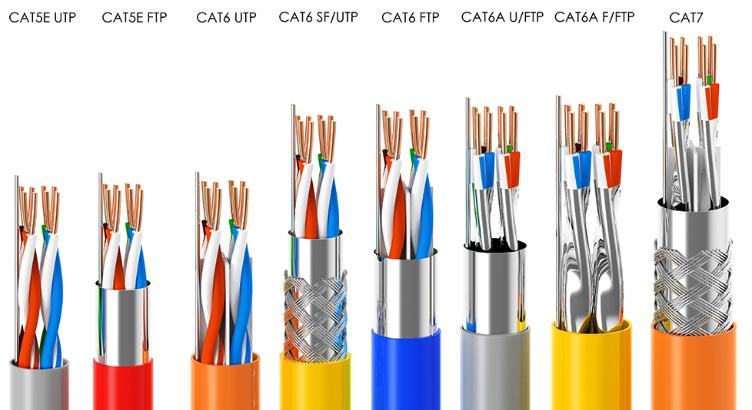
\includegraphics[width=1\textwidth]{./figuras/cables_cat}
\caption{Cables Cat con sus diferentes trenzados y apantallamientos\cite{i_cables}.}
\label{F:cables_cat}
\end{center}
\end{figure}

Como la conexión principal con el ISP actualmente de los diferentes domicilios/locales oscila entre 300-1000 Mbps, ha prevalecido el uso de Giga ethernet sobre Ethernet para permitir un uso maximizado de la conexión, pero no se han utilizado routers o switch 2.5Gbps, ni protocolos Wifi6, que permiten velocidades superiores a Giga ethernet debido a los aumentos de los costes. 

\subsection{Switch}
Tanto para la instalación de la oficina física, como el cableado de diferentes viviendas, incluso ciertos proyectos personales se han usado una multitud de switch entre los que destacan los siguientes modeles giga ethernet:

\subsubsection{TP-LINK TL-SG108 Switch 8 Puertos}
Especialmente utilizado como switch principal, administrado y configurado con VLAN, perfecto para cablear una oficina o casa, figura \ref{F:giga_switch_8p}.
\begin{figure}[htbp]
\begin{center}
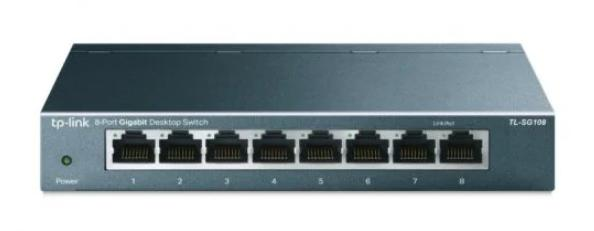
\includegraphics[width=0.8\textwidth]{./figuras/giga_switch_8p}
\caption{Imagen TP-LINK TL-SG108 Switch 8 Puertos (PCComponent imágenes).}
\label{F:giga_switch_8p}
\end{center}
\end{figure}
\subsubsection{TP-Link LS1005G Switch 5 Puertos Gigabit}
Adecuado como una versión inferior, con menor cantidad de puertos,figura \ref{F:giga_switch_5p}.
\begin{figure}[htbp]
\begin{center}
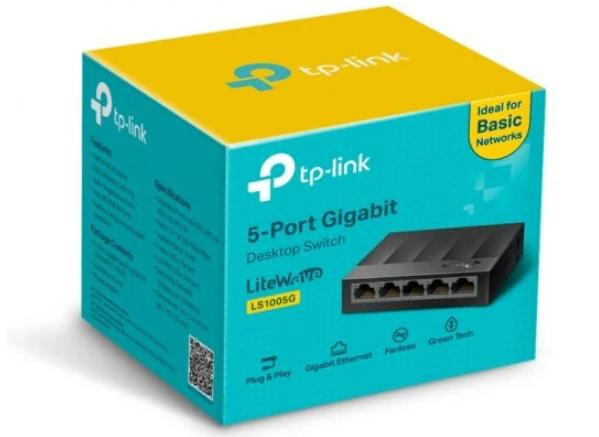
\includegraphics[width=0.8\textwidth]{./figuras/giga_switch_5p}
\caption{Imagen TP-Link LS1005G Switch 5 Puertos (PCComponent imágenes).}
\label{F:giga_switch_5p}
\end{center}
\end{figure}
\subsubsection{Mercusys MS105G Switch 5 Puertos Gigabit}
Low cost giga switch, perfecto para redistribución de elementos conectado en la propia oficina, así como wake up o alimentación por ethernet, figura \ref{F:lowcost_giga_switch}.
\begin{figure}[htbp]
\begin{center}
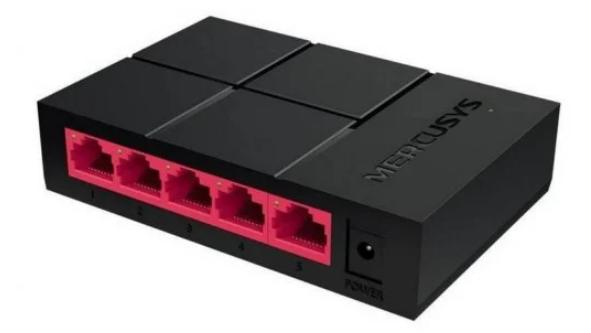
\includegraphics[width=0.8\textwidth]{./figuras/lowcost_giga_switch}
\caption{Imagen Mercusys MS105G Switch 5 Puertos (PCComponent imágenes).}
\label{F:lowcost_giga_switch}
\end{center}
\end{figure}

\subsection{Router}
Actualmente cualquier router WLAN-LAN en un presupuesto 20€-60€, incluye un puerto WLAN giga ethernet(azul), al menos 4 o mas puertos giga ethernet LAN, un hotspod wifi con protocolo 802.11n o superiores y permite la configuración de múltiples modos:
\begin{itemize}
    \item Modo Router-Broker, genere comunicación entre WLAN, LAN y la WLAN generadas. Tiene servicio DHCP y permite la configuración estática manual (filtros, IPs, tabla de rutas.
    \item Modo NAT-LAN, similar al anterior genera un LAN y un WLAN interconectadas pero separadas por VLAN, todas ellas con una NAT-MASQUERADE hacia la WLAN que provee de internet. Es equivalente a un router ADSL o fibra.
    \item Modo wireless WAN, es decir conectarse a otro router de manera inalámbrica que actúa de WAN.
    \item Modo Repetidor, permite extender las funcionalidades de una LAN/WLAN ya existente (vía cable o wireless).
    \item Muchos de ellos incluyen 1 o 2 USB, con perspectivas a servicios que requieren almacenamiento o para la interconexión de router-3G/4G como fuente de conectividad en caso de desconexión del puerto WLAN.
\end{itemize}

Por otra parte suelen incluir múltiples servicios externos tales como:
\begin{itemize}
    \item[--] Clientes VPN, especialmente openVPN y wireguard o derivados. Algunos también incluyen API de clientes VPN de proveedores externos basados en protocolos estándares.
    \item[--] Clientes DynamicDNS, son principales clientes de redirección de dominios dns, que se actualizan para permitir apuntar a un IP dinámica desde internet.
    \item[--] DMZ, firewall filtrado o redirección de puertos, IPv6, servidor multimedia (ftp, vídeo), e incluso servidores vozip configuración de asterix y otros servicios relacionados con multimedia dentro de una LAN.
\end{itemize}

Se han utilizado múltiples modelos de routers especialmente Linksys E5400-EU Router WiFi AC, Xiaomi Mi Router WiFi AC y Asus RT-AX53U Router WiFi 6, así como algún que otro modelo genérico chino de aliexpress.

Las principales funcionalidades de estos router son basadas en software, es decir, en muchos casos con formatear y cambiar el software embeded del router a versiones como dd-wrt\cite{c_dd_wrt} habilita una mejor gestión y mas posibilidades especialmente en clientes VPN y enrutado customizable.

\subsubsection{Router Portable}
Un router portable es básicamente un dispositivo similar a una rasberry pi o placas similares o un router especialmente reducido. Usualmente cuenta con 1 o 2 puertos ethernet, un usb para interconectar router 3G/4G o directamente slot para sim.
\begin{figure}[!htbp]
\begin{center}
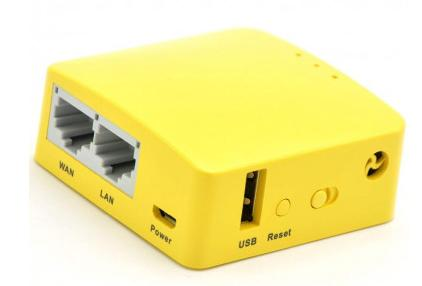
\includegraphics[width=0.7\textwidth]{./figuras/router_portable}
\caption{Router portable GL-MT300N-V2 (amazon products).}
\label{F:router_portable}
\end{center}
\end{figure}
Similar a los router WAN, permite la interconexión por cable, wireless o moden telefónico y dispone especialmente de conectores VPN-cliente, NAT-Masquerade y la configuración customizada de filtros, rutas y otras herramientas de diagnostico. En muchos casos se alimenta vía USB o 5V, con reducidos consumos, la antenas son co-planar embeded y no tiene una cobertura muy amplio (10-20 m).

Su principal función es ser configurados (sus clientes y parámetros internos) para se 'desplegados' de manera portable usualmente por Cable Ethernet o conexión móvil (3G/4G) aunque también permite conectarse a hotspot wireless. Su bajo consumo permite a su vez desplegarlo con un powerbank durante varias horas.

La principal ventaja de este route es su portabilidad y movilidad, es decir, permite de una manera practica utilizarlo como router con vpn integrada en cualquier LAN a la que se conecte físicamente, facilitando la configuración de un entorno seguro en cualquier acceso con a internet median rj45.

\subsection{Servidor autocrático}
Los servidores autocráticos son por definición servidores en casa o en la oficina, permiten un uso mayor de recursos aunque la 'availability' de sus recursos se ve resentida por la red eléctrica y la conexión de comunicaciones de la sede en la que se sitúan.

Por otra parte esta el tema de gasto eléctrico; para evitar un consumo eléctrico mayor al coste de un servidor en la nube o dedicado es necesario limitar la potencia del servidor o las horas encendido.

Existen varias estrategias:
\begin{itemize}
    \item Hardware especializado, que tiene bajo consumos en momento de baja actividad.
    \item Utilización de mini-pc con bajos consumos 6-10 W (CPU N100 , N300) o plataformas arm como raspberry pi o similares 1-6W. 
    \item Encendidos y apagados programados basado en un scheduler y demanda de trabajo por realizar.
\end{itemize}

En todas ellas el objetivo es un coste reducido o en función del trabajo realizado, y es factible la combinación de más de una solución con el fin de no perjudicar el principal activo que es la mayor disponibilidad de recursos en el servidor autocrático que un VPS.

\subsubsection{Arm servers}
Debido a la naturaleza de bajo coste y especialmente bajo consumo las placas basados en arm son perfectas para servidores low cost con consumos de 1-6 w.

\begin{figure}[!htb]
\begin{center}
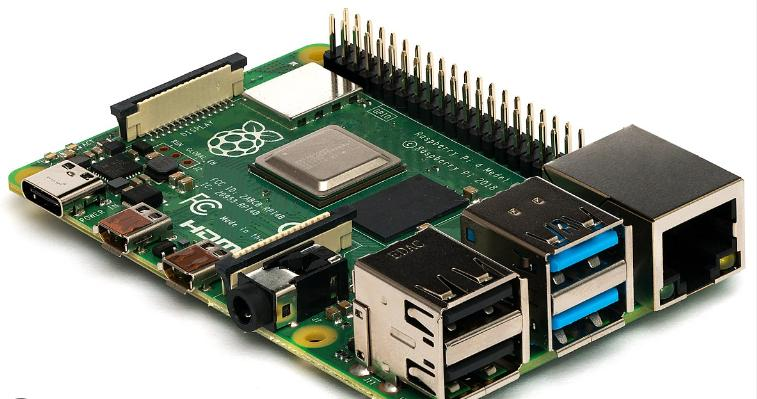
\includegraphics[width=0.7\textwidth]{./figuras/rasberripi}
\caption{Placa Rasberry pi (amazon products imagen).}
\label{F:rasberripi}
\end{center}
\end{figure}
\begin{figure}[!htbp]
\begin{center}
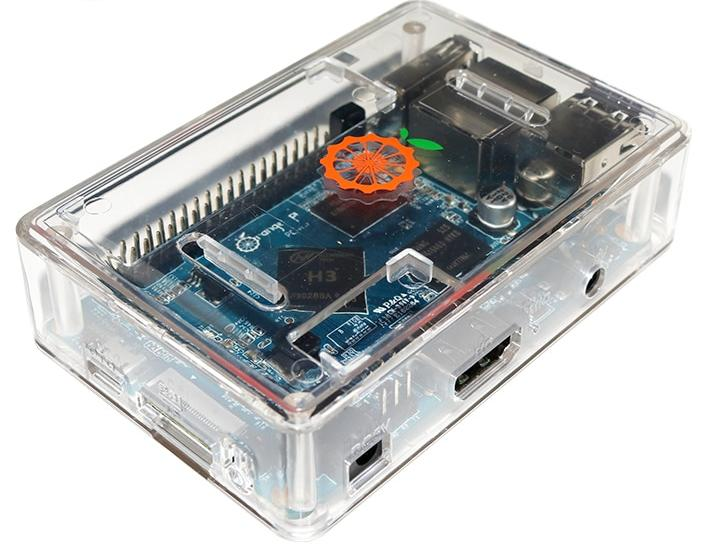
\includegraphics[width=0.7\textwidth]{./figuras/orangepi_pc}
\caption{Placa Orange Pi PC 3 (Aliexpress products imagen).}
\label{F:orangepi_pc}
\end{center}
\end{figure}
En las implementaciones de los diversos proyectos donde se ha aplicado este documento se han utilizado múltiples versiones, todas ellas basadas en rasberri pi OS, raspbian (custom debian para rasberry pi), ubuntu/fedora/debian arm versión, armbian (custom debian para arm boards) entre otros.

Así mismo se han utilizado placas Rasberry pi V1, V2, V3, junto a otras placas similares OrangePi Pc3, BananaPI M2+, en cada uno de los domicilios o sedes donde existen servidores autocráticos, elementos de red, interconexiones LAN-VPN o directamente como servidor autocrático en si.
\begin{figure}[!htbp]
\begin{center}
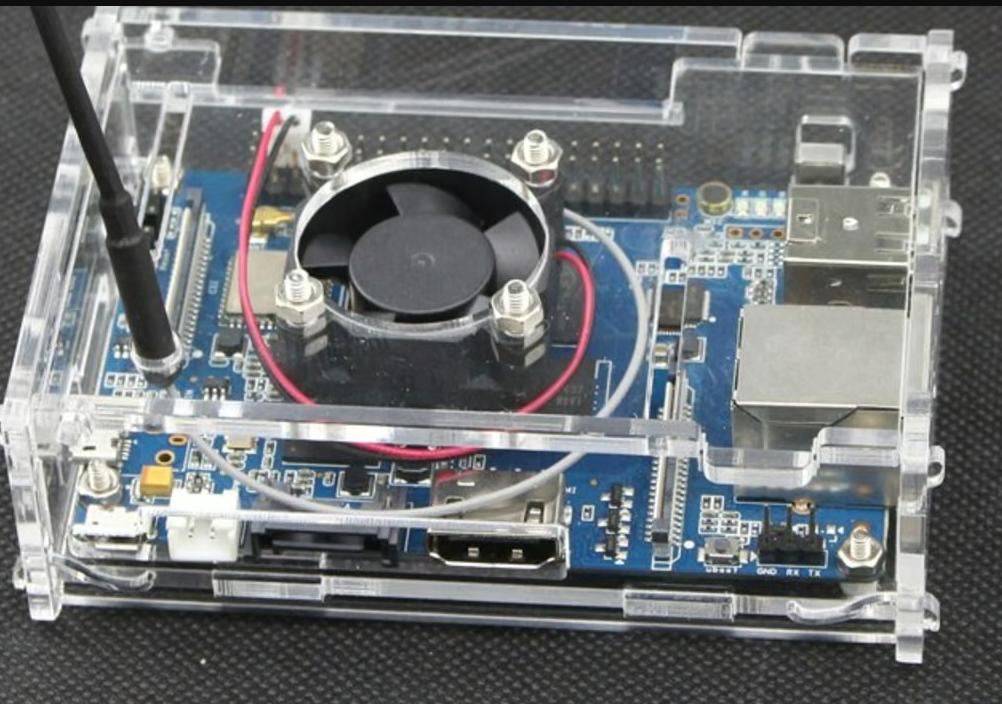
\includegraphics[width=0.7\textwidth]{./figuras/bananapi}
\caption{Placa Banana Pi M2+(Aliexpress products imagen).}
\label{F:bananapi}
\end{center}
\end{figure}

\subsubsection{Noc server}
Aquellos casos que se requiere de un servidor de recursos aceptables y especialmente procesador X86-64, es decir, para ejecutar servicios dockerizados no especializados en plataforma arm. Se han seleccionado mini-pc con los CPU N100-N305 con consumo de 6-15W pero la potencia en recursos de un ordenador de 2010-15.
\begin{figure}[!htbp]
\begin{center}
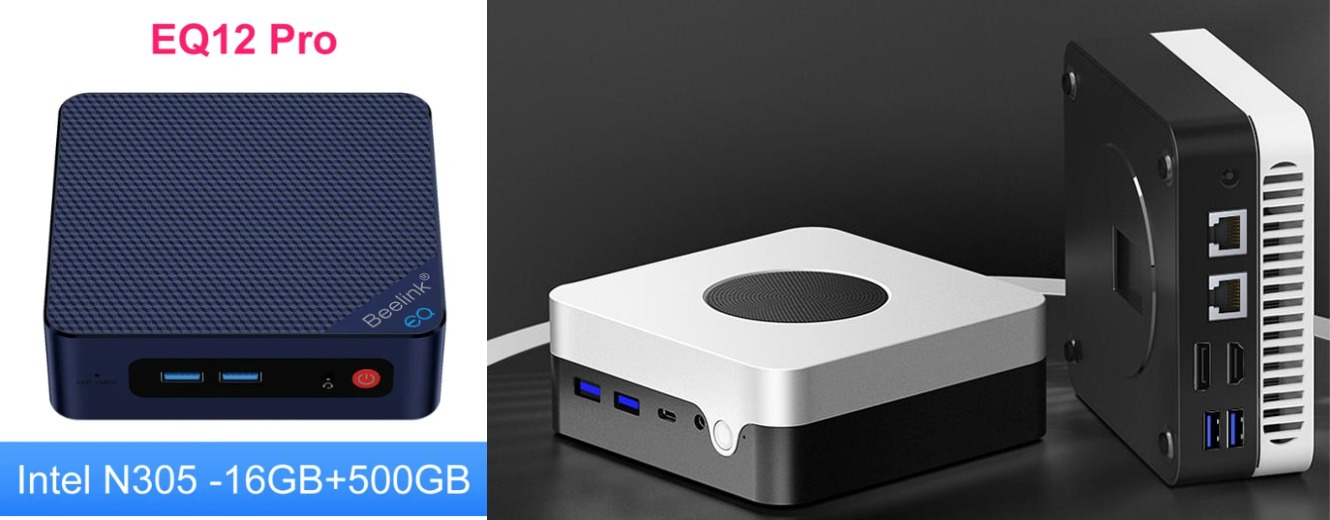
\includegraphics[width=1\textwidth]{./figuras/minipc}
\caption{EQ12 Pro y Chuwi LarkBox X (Aliexpress products imagen).}
\label{F:minipc}
\end{center}
\end{figure}

\subsubsection{PC y portátiles viejos}
Un gran abanico de antiguos portátiles o torres, semi actualizadas pueden ser utilizados como servidores temporales, es decir fuente de recursos encendidos remotamente para por ejemplo mediante ansible setear un cluste de docker swarm o kubernetes con propósitos de pruebas y desarrollo, para ser apagado después de su uso.

\subsection{Camaras IP}
Se dispone de una amalgama de cámaras IP la gran mayoría con imagen normal, infrarrojo, sonido y altavoz sobre el actuar. Así como motorizadas 360º o con seguimiento de humanos, tanto interiores como exteriores; todas con costes entre los 10€-60€ (low cost).

La principal característica dentro de este documento es el uso de VPS-VPN para centralizar y permitir un acceso ágil a las IP cam, permitiendo usar software dockerizado para la monitorización y generación de flujow de vídeo, tanto para almacenamiento como para procesado de imágenes. Todas la cámaras IP se sitúan en zonas privadas, por lo que la regulación de no es aplicable y tiene un carácter preventivo de seguridad.

El uso de esta VPN e interconexión de fuentes ipcam con servicios dockerizados que las utilizan, permite evadir el uso de las aplicaciones nativas de dichas cámaras, usualmente con fallos de seguridad y blindar el firewall de las diferentes LAN, para evitar tener ataques reversos a través de las cámaras ip, con software no parcheado.

Por ultimo, el relego de la generación de diferentes señales Wireless en cada LAN, especialmente en el caso de las ipcam, con el objetivo de separar compartimentando, pero especialmente evitando degradar la señal de la WLAN como el protocolo usado debido a enlaces de datos degradados (ipcam-router). 

\subsection{Smart Devices}

Se han utilizado diferentes elementos inteligentes o red de sensores, focalizado en demótica o acciona-dores. Como elementos principales destacan el uso de Alexa / Google Home como interfaz audio-vocal y gateways vía bluetooth o WIFI, así como la instalación de gateways de zigbee, z-wave o sensores a 144 Mhz.

Inicialmente se buscaba una interacción entre diversos elementos, luces, sensores y acciones para elementos de la oficina tales como, luz, temperatura, y automatismos. Sin embargo en un segunda revisión como proyecto personal involucro la seguridad y monitorización de elementos como el consumo eléctrico, para finalmente también añadir actuadores.

Como conclusión se han utilizado una plataforma de sensores y actuadores (incluyendo alarma y centralita) basada en Gautone, plataformas Alexa / google home, la interconexión de diversos electrodomésticos todo ello centralizado por una rasberry pi con Home Assistan, que es el elemento que a través de autenticación de token API en las otras plataformas, permite unir transversalmente todos los elementos, aísla o federa-liza los recursos de las API bajo un criterio mas seguro y privado.

Destaco por su sencillez y bajo coste:
\begin{itemize}
    \item Sensores magnéticos, sensores de presencia, sensor de temperatura y humedad.
    \item Sensor-adicionador termostato (accesible y programable vía nube), luces, enchufes inteligentes o conmutadores, así como PIA conectados.
    \item La facilidad de integración de sensores propios vía placas ESP32 o rasberry en API  de terceros.
\end{itemize}